\subsection{Geometrical ellipsoids}

For our purposes, it is useful to give ellipsoids a general definition that includes, in addition to the usual proper ellipsoid that is bounded with non-empty interior,  ellipsoids that may be unbounded in some directions and singular ellipsoids that are flat with empty interior.
% Being a unit ellipsoid is not an intrinsic property of the ellipsoid but only relative to either a distribution for which
% it represents quadratic dispersion or with respect to a norm or inner product for which it is the unit sphere.
% Since there is no clear reference at this stage for the ellipsoid to be a unit ellipsoid it seemed easier to me to
% hold off until we talk about the ellipsoid for a distribution. Presumably we want to avoid references to norms
% and inner products.
%
% To make the statements correct in their full elegant generality, we unfortunately need to be more explicit about
% singular and unbounded ellipsoids.
% The implicit definition: x'Cx = 1 doesn't generate singular ellipsoids, for that we need transformations.
% Transformations on the other hand don't generate unbounded ellipsoid.
% For that we need a positive semi-definite C.  I've tried to
% weave both representations to avoid excessive formality and to encourage visualization.
% Instead of 'unbounded' and 'degenerate' ellipsoids, I refer to improper and singular ellipsoids because these terms
% seem more consonant with terms for the distributions to which they correspond.  I therefore use 'proper' ellipsoid for
% a bounded ellipsoid with non-empty interior.
%
% I can reedit this to make it more consistent with the following material
%

A proper ellipsoid in the $p$-dimensional space $\Real{p}$
%$\Re^p$
centered at the origin, $\vec{0}$,
may be defined by the quadratic form
\begin{equation}\label{eq:ellisoid1}
\mathcal{E} := \{ \vec{x}: \vec{x}\trans \mat{C} \vec{x} =1 \} \comma
\end{equation}
where $\vec{x} = (x_1, x_2, \dots , x_p)\trans$ is a vector referring to the coordinate axes and $\mat{C}$ is a symmetric
positive definite $p \times p$ matrix.
If $\mat{C}$ is positive semi-definite then the ellipsoid will be ``improper,'' having the shape of a cylinder with elliptical cross-sections and unbounded in the direction of the null space of $\mat{C}$.
To extend the definition to singular (sometimes known as ``degenerate'') ellipsoids, we turn to a definition that is equivalent to \eqref{eq:ellisoid1} for proper ellipsoids.
Let $\mathcal{S}$ denote the unit sphere in  $\Real{p}$,
\begin{equation}
\mathcal{S} := \{ \vec{x}: \vec{x}\trans\vec{x} =1 \} \comma
\end{equation}
and let
\begin{equation}\label{eq:ellisoidsph}
\mathcal{E} := \mat{A} \mathcal{S} \comma
\end{equation}
where $\mat{A}$ is a non-singular $p \times p$ matrix. Then $\mathcal{E}$ is a proper ellipsoid that could be defined using \eqref{eq:ellisoid1} with $\mat{C} = \left( \mat{A} \trans \mat{A} \right)^{-1}$.
We obtain singular ellipsoids by allowing $\mat{A}$ to be any matrix, not necessarily non-singular nor even square.
Some useful properties are:
\begin{figure}[tb]
  \centering
  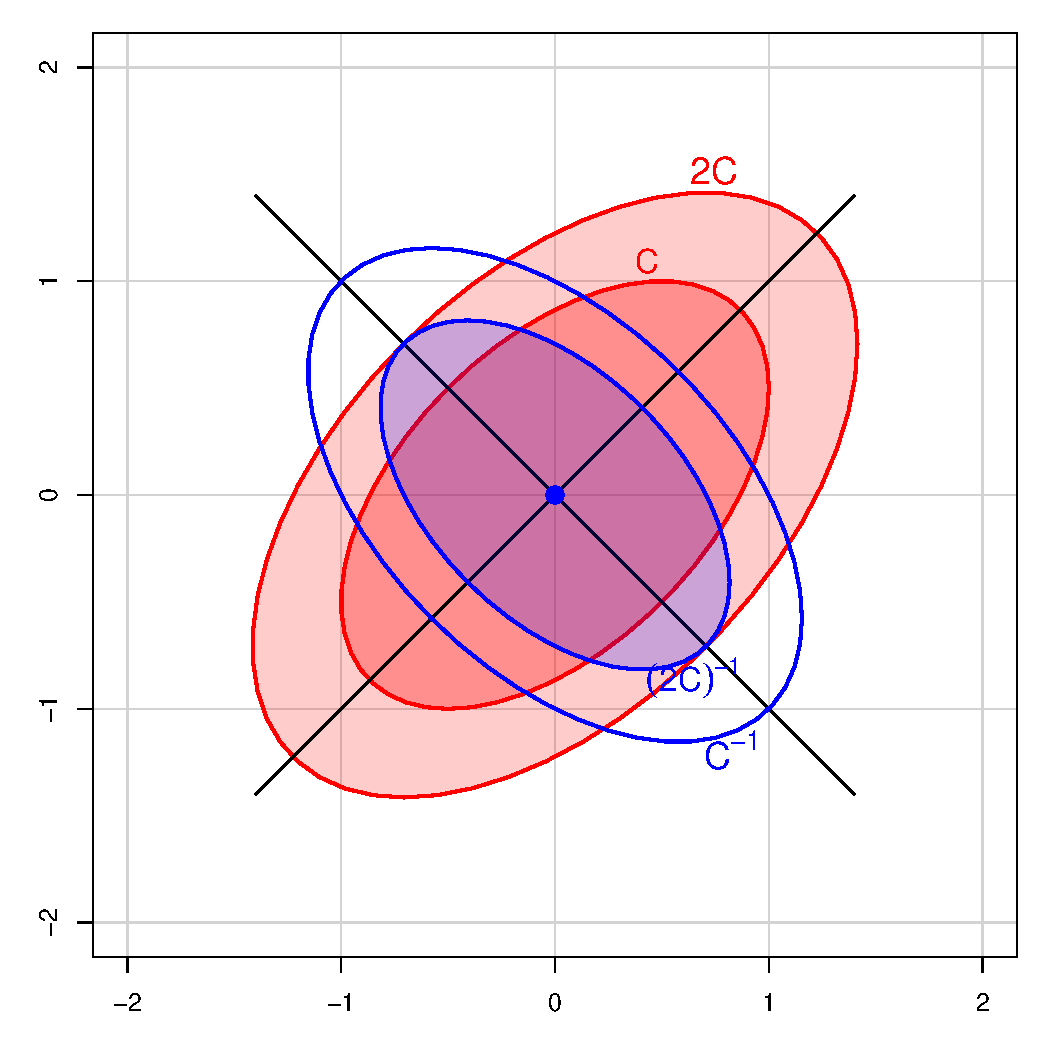
\includegraphics[width=.5\textwidth,clip]{fig/inverse}
  \caption{Some properties of geometric ellipsoids. Principal axes of an ellipsoid are given by the eigenvectors of
  $\mat{C}$, with radii $1/\sqrt{\lambda_i}$.  For an ellipsoid defined by \eqref{eq:ellisoid1},
  the comparable ellipsoid for $2\mat{C}$ has radii multiplied by $1/\sqrt{2}$.
  The ellipsoid for $\mat{C}^{-1}$ has the same principal axes, but with radii $\sqrt{\lambda_i}$, making it
  small in the directions where $\mat{C}$ is large and vice-versa.
  } \label{fig:inverse}
\end{figure}

\begin{itemize}
 \item Translation: An ellipsoid centered at $\vec{x}_0$ has the definition $\mathcal{E} := \{ \vec{x}: (\vec{x}-\vec{x}_0)\trans \mat{C} (\vec{x}-\vec{x}_0) =1 \}$ or $\mathcal{E} := \mat{A} \mathcal{S} + \vec{x}_0$.

 \item Orthogonality: If $\mat{C}$ is diagonal, the origin-centered ellipsoid has its axes aligned with the coordinate axes, and
has the equation
\begin{equation}\label{eq:ellisoid2}
 \vec{x}\trans \mat{C} \vec{x} = c_{11} x_1^2 + c_{22} x_2^2 + \cdots + c_{pp} x_p^2 =1 \comma
\end{equation}
where $1/\sqrt{c_{ii}} = c_{ii}^{-1/2}$ are the radii (semi-diameter lengths) along the coordinate axes.

 \item Area and volume: In two dimensions, the area of the axis-aligned ellipse is $\pi (c_{11} c_{22})^{-1/2}$.
 For $p=3$, the volume is $\frac{4}{3}\pi (c_{11} c_{22} c_{33})^{-1/2}$.
 In the general case, the hypervolume of the ellipsoid is proportional to $|\mat{C}|^{-1/2}=||\mat{A}||$
 and is given by $\pi^{p/2} / \left[ \det{\mat{C}}^{1/2} \Gamma\left(\frac{p}{2}+1\right) \right]$.

 \item Principal axes: In general, the eigenvectors, $\vec{v_i}, i=1,\dots,p$,
of $\mat{C}$ define the principal axes of the ellipsoid and
the inverse of the square roots of the ordered
eigenvalues, $\lambda_1 > \lambda_2 \dots, \lambda_p$, are the principal radii.
Eigenvectors belonging to eigenvalues that are 0 are directions in which the ellipsoid is unbounded.
With $\mathcal{E} = \mat{A} \mathcal{S}$, we consider the singular-value decomposition
$  \mat{A}= \mat{U} \mat{D} \mat{V} \trans$,
with $\mat{U}$ and  $\mat{V}$ orthogonal matrices and  $\mat{D}$  a diagonal non-negative matrix
with the same dimension as $\mat{A}$.
The column vectors of $\mat{U}$, called the left singular vectors,
correspond to the eigenvectors of $\mat{C}$ in the case of a proper ellipsoid.
The positive diagonal elements of $\mat{D}$, $d_1 > d_2 > ... > d_p>0$,
are the principal radii of the ellipse with $d_i = 1/\sqrt{\lambda_i}$.
In the singular case, the left singular vectors form a set of principal axes for the flattened ellipsoid.\footnote{Corresponding left singular vectors and eigenvectors are not necessarily equal but sets that belong to the same eigenvalue/singular value span the same space.}

 \item Inverse: When $\mat{C}$ is positive definite, the eigenvectors of \mat{C} and $\mat{C}^{-1}$ are identical, while
the
 eigenvalues of $\mat{C}^{-1}$ are $1/\lambda_i$. It follows that the ellipsoid for
 $\mat{C}^{-1}$ has the same axes as that of $\mat{C}$, but with inversely proportional radii.
 In $\Real{2}$, the ellipsoid for $\mat{C}^{-1}$
 is, with rescaling, a \degree{90} rotation of the ellipsoid for $\mat{C}$,
 as illustrated in \figref{fig:inverse}.

 \item Generalized inverse: A definition for an inverse ellipsoid that is equivalent in the case of proper ellipsoids,
\begin{equation}\label{eq:ellipseginv}
\mathcal{E}^{-1} = \{ \vec{y} :   |\vec{x} \trans \vec{y}| \le 1 \comma \quad \forall \vec{x} \in \mathcal{E} \} \comma
\end{equation}
generalizes to all ellipsoids. The inverse of a singular ellipsoid is an improper ellipsoid and vice versa.

 \item Dimensionality: The ellipsoid is bounded if $\mat{C}$ is positive definite (all $\lambda_i > 0$).
 Each $\lambda_i = 0$ increases the dimension of the space along which the ellipsoid is unbounded by one.
For example, with $p=3$, $\lambda_3=0$ gives a
cylinder with an elliptical cross-section in 3-space, and  $\lambda_2 = \lambda_3=0$ gives an infinite slab with thickness $2 \sqrt{\lambda_1}$. With $\mathcal{E} = \mat{A} \mathcal{S}$, the dimension of the ellipsoid is equal to the number of positive singular values of $\mat{A}$.
 \item Projections: The projection of a $p$ dimensional ellisoid into any subspace
is $\mat{P} \mathcal{E}$, where
$\mat{P}$ is an idempotent $p \times p$ (projection) matrix, i.e., $\mat{P} \mat{P}= \mat{P}^2 = \mat{P}$.
For example, in $\Real{2}$ and $\Real{3}$,
% $\Re^3$,
the matrices
\[
\mat{P}_2 =
\left[
\begin{array}{cc}
 1 & 1  \\
 0 & 0  \\
\end{array}
\right]
\comma \quad\quad
\mat{P}_3 =
\left[
\begin{array}{ccc}
 1 & 0 & 0 \\
 0 & 1 & 0 \\
 0 & 0 & 0 \\
\end{array}
\right]
\]
project, respectively, an ellipse onto the line $x_1 = x_2$, and an ellipsoid into the ($x_1, x_2$) plane.  If $\mat{P}$ is symmetric, then $\mat{P}$ is the matrix of an orthogonal projection, and it is easy to visualize  $\mat{P} \mathcal{E}$ as the shadow of  $\mathcal{E}$ cast perpendicularly onto  $\mathrm{span}(\mat{P})$. Generally,  $\mat{P} \mathcal{E}$ is the shadow of $\mathcal{E}$  onto  $\mathrm{span}(\mat{P})$ along the null space of $\mat{P}$.

 \item Linear transformations: A linear transformation of an ellipsoid is an ellipsoid, and the pre-image of an ellipsoid under a linear transformation is an ellipsoid.  A non-singular linear transformation maps a proper ellipsoid into a proper ellipsoid.

 \item Slopes and tangents: The slopes of the ellipsoidal surface in the directions of the coordinate
 axes are given by $\partial / \partial \vec{x} \: (\vec{x}\trans \mat{C} \vec{x}) = 2 \mat{C} \vec{x}$.
 From this, it follows that the tangent hyperplane to the unit ellopsoidal surface at the point
 $\vec{x}_\alpha$, where $\vec{x}_\alpha\trans \: \partial / \partial \vec{x} (\vec{x}\trans \mat{C} \vec{x}) = 0$,
 has the equation $\vec{x}_\alpha \trans \mat{C} \vec{x} = 1$.
\end{itemize}

